\documentclass[10pt,a4paper]{article}
\usepackage[utf8]{inputenc}
\usepackage[T1]{fontenc}
\usepackage{lmodern,microtype}
\usepackage[a4paper,margin=1.65cm]{geometry}
\usepackage{amsmath,amssymb,booktabs,tabularx,longtable,graphicx,float,array}
\usepackage[hidelinks]{hyperref}
\newcolumntype{Y}{>{\raggedleft\arraybackslash}X}
\title{Supplementary Material\\Forecasting annual counts of large wildfires in Spain}
\author{Santi García-Cremades, José Juan López Espín, José María Cecilia Canales}
\date{}
\begin{document}
\maketitle

\section{Reproducibility map}
\begin{table}[H]\centering\footnotesize
\begin{tabularx}{\textwidth}{p{4.9cm}X}
\toprule
File & Purpose \\
\midrule
\path{analisis_clasico_arima_arimax_v13.py} & Prespecified ARIMA grid, AutoReg models, exponential smoothing, Holt, ARIMAX lag sensitivity, fit and predictive $R^2$, relative skill and sequential external validation. \\
\path{modelos_conteo_gif_v13.py} & NB2 observation-driven models, Bayesian negative-binomial AR(1), rolling-origin validation, probabilistic metrics and external validation. \\
\path{analysis_prospective_2026.py} & Frozen 2026 ARIMA prediction, dated MITECO snapshot, historical same-date completion benchmark and conditional lag-two heat-exposure scenarios. \\
\bottomrule
\end{tabularx}
\end{table}

\section{Response overdispersion}
For 2005--2023, $n=19$, mean $=25.684$, variance $=319.006$, variance-to-mean ratio $=12.420$, minimum $=3$ and maximum $=58$. The Bayesian parameterisation uses $\operatorname{Var}(N\mid\mu,\alpha)=\mu+\mu^2/\alpha$, whereas the frequentist NB2 parameterisation uses $\mu+\phi\mu^2$.

\section{Complete classical benchmark}
The constant-only ARIMA$(0,0,0)$ and the unstable highest-order specification were excluded a priori. Rolling-origin errors, rather than in-sample AICc alone, determined the benchmark.

\subsection{ARIMA grid}
\begin{longtable}{lrrrrrr}
\toprule
Model & $n$ & MAE & RMSE & NMAE & MASE & $R^2_{\mathrm{pred}}$ \\
\midrule
\endfirsthead
\toprule
Model & $n$ & MAE & RMSE & NMAE & MASE & $R^2_{\mathrm{pred}}$ \\
\midrule
\endhead

ARIMA$(1,0,0)$ & 10 & 12.84 & 18.81 & 0.556 & 0.616 & -0.177 \\
ARIMA$(2,0,0)$ & 10 & 14.30 & 19.44 & 0.619 & 0.686 & -0.258 \\
ARIMA$(0,0,1)$ & 10 & 14.61 & 18.52 & 0.633 & 0.701 & -0.142 \\
ARIMA$(2,0,1)$ & 10 & 15.46 & 19.54 & 0.669 & 0.742 & -0.271 \\
ARIMA$(0,1,1)$ & 10 & 15.66 & 21.32 & 0.678 & 0.752 & -0.512 \\
ARIMA$(2,1,1)$ & 10 & 16.01 & 22.26 & 0.693 & 0.769 & -0.649 \\
ARIMA$(1,1,1)$ & 10 & 16.08 & 22.18 & 0.696 & 0.772 & -0.637 \\
ARIMA$(1,0,1)$ & 10 & 16.44 & 20.95 & 0.712 & 0.789 & -0.461 \\
ARIMA$(0,0,2)$ & 10 & 17.06 & 22.13 & 0.739 & 0.819 & -0.630 \\
ARIMA$(3,0,0)$ & 10 & 17.52 & 20.70 & 0.758 & 0.841 & -0.426 \\
ARIMA$(1,0,2)$ & 10 & 19.26 & 24.10 & 0.834 & 0.924 & -0.932 \\
ARIMA$(2,1,0)$ & 10 & 19.46 & 25.18 & 0.843 & 0.934 & -1.111 \\
ARIMA$(2,0,3)$ & 9 & 20.22 & 26.09 & 0.812 & 0.971 & -1.255 \\
ARIMA$(2,1,2)$ & 10 & 20.34 & 28.12 & 0.880 & 0.976 & -1.632 \\
ARIMA$(3,1,2)$ & 9 & 20.40 & 29.81 & 0.820 & 0.979 & -1.944 \\
ARIMA$(0,1,2)$ & 10 & 20.78 & 27.41 & 0.899 & 0.997 & -1.500 \\
ARIMA$(1,1,0)$ & 10 & 20.80 & 25.78 & 0.901 & 0.999 & -1.211 \\
ARIMA$(3,1,0)$ & 10 & 22.27 & 30.37 & 0.964 & 1.069 & -2.070 \\
ARIMA$(3,0,2)$ & 9 & 22.29 & 25.72 & 0.896 & 1.070 & -1.192 \\
ARIMA$(3,0,1)$ & 10 & 22.30 & 25.90 & 0.965 & 1.070 & -1.232 \\
ARIMA$(1,1,2)$ & 10 & 22.82 & 28.48 & 0.988 & 1.095 & -1.700 \\
ARIMA$(1,0,3)$ & 10 & 23.32 & 26.43 & 1.009 & 1.119 & -1.325 \\
ARIMA$(0,1,0)$ & 10 & 23.34 & 31.56 & 1.010 & 1.120 & -2.315 \\
ARIMA$(1,1,3)$ & 10 & 23.45 & 34.82 & 1.015 & 1.126 & -3.035 \\
ARIMA$(0,1,3)$ & 10 & 23.91 & 30.92 & 1.035 & 1.148 & -2.182 \\
ARIMA$(3,1,1)$ & 10 & 24.23 & 32.85 & 1.049 & 1.163 & -2.592 \\
ARIMA$(0,0,3)$ & 10 & 24.63 & 28.60 & 1.066 & 1.182 & -1.723 \\
ARIMA$(2,1,3)$ & 9 & 24.90 & 35.94 & 1.000 & 1.195 & -3.279 \\
ARIMA$(3,0,3)$ & 8 & 32.05 & 37.86 & 1.233 & 1.538 & -3.363 \\
ARIMA$(2,0,2)$ & 10 & 46.30 & 85.44 & 2.004 & 2.222 & -23.295 \\
\bottomrule
\end{longtable}

\subsection{Non-ARIMA references}
\begin{table}[H]\centering\small
\begin{tabular}{lrrrrrr}
\toprule
Model & $n$ & MAE & RMSE & NMAE & MASE & $R^2_{\mathrm{pred}}$ \\
\midrule
Damped Holt & 10 & 12.56 & 19.26 & 0.544 & 0.603 & -0.234 \\
AutoReg(2) & 10 & 13.69 & 17.53 & 0.593 & 0.657 & -0.022 \\
AutoReg(1) & 10 & 14.25 & 18.69 & 0.617 & 0.684 & -0.162 \\
Additive Holt & 10 & 14.72 & 21.28 & 0.637 & 0.706 & -0.507 \\
AutoReg(3) & 10 & 14.82 & 17.99 & 0.641 & 0.711 & -0.077 \\
Simple exponential smoothing & 10 & 15.31 & 18.41 & 0.663 & 0.735 & -0.128 \\
Historical mean & 10 & 15.31 & 18.41 & 0.663 & 0.735 & -0.128 \\
Naive & 10 & 20.40 & 26.75 & 0.883 & 0.979 & -1.381 \\
\bottomrule
\end{tabular}
\end{table}

\begin{figure}[H]\centering
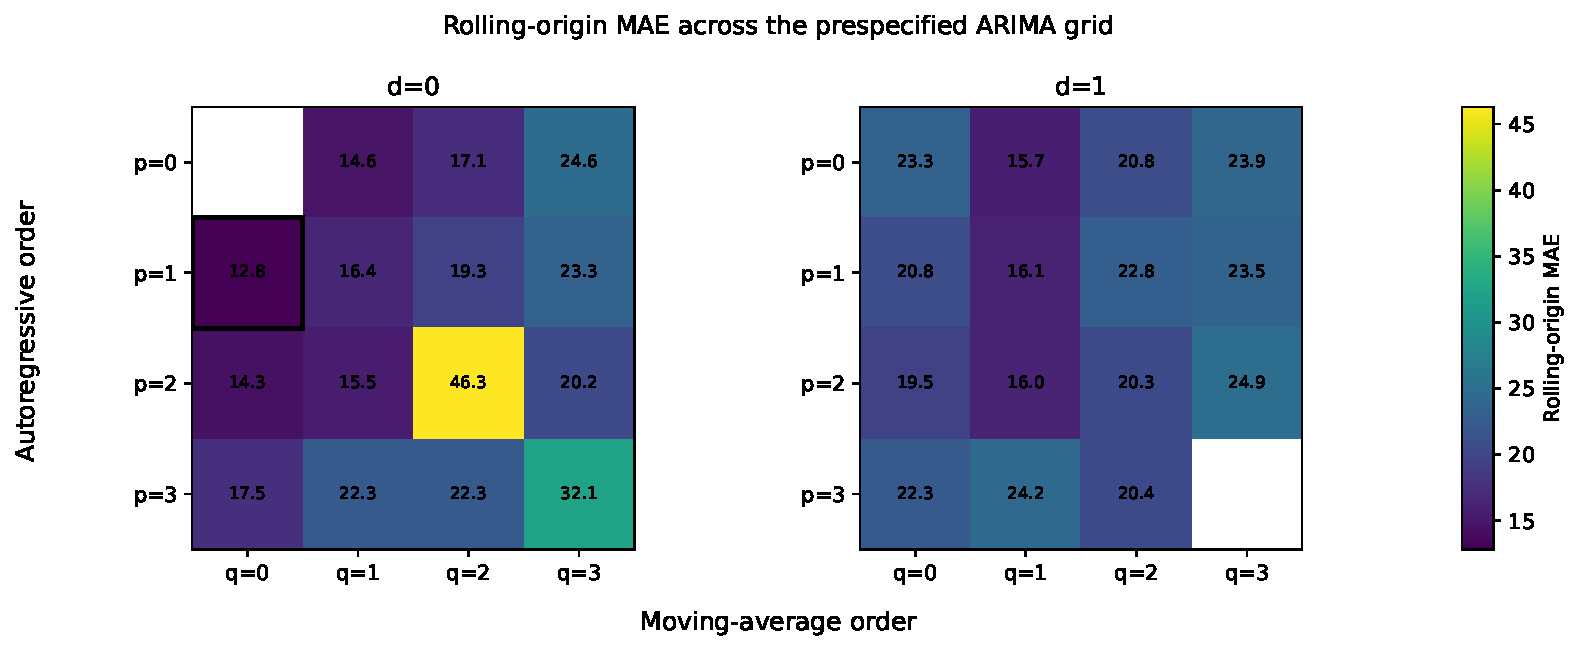
\includegraphics[width=0.86\textwidth]{../figures/figS1_arima_grid.pdf}
\caption{Rolling-origin MAE across the prespecified ARIMA grid. ARIMA$(1,0,0)$ is outlined.}
\end{figure}

Negative predictive $R^2$ values are valid: they mean that the squared forecast error exceeded the error of using the validation-window mean. They are not retrospective coefficients of determination.

\section{ARIMAX lag sensitivity and coefficients}
\begin{table}[H]\centering\small
\begin{tabular}{lrrrrrr}
\toprule
Specification & MAE & RMSE & $R^2_{\mathrm{pred}}$ & MSE skill & $p_H$ & $p_P$ \\
\midrule
Heat + prevention $(t-1)$ & 10.32 & 12.93 & 0.491 & 0.597 & 0.061 & 0.175 \\
Heat + prevention $(t-2)$ & 16.83 & 25.06 & -0.911 & -0.511 & 0.001 & 0.010 \\
Heat + prevention $(t-3)$ & 8.79 & 13.37 & 0.456 & 0.570 & 0.013 & 0.332 \\
Heat only & 9.64 & 12.85 & 0.497 & 0.602 & 0.099 & --- \\
ARIMA$(1,0,0)$ & 13.97 & 20.38 & -0.265 & 0.000 & --- & --- \\
\bottomrule
\end{tabular}
\end{table}

The lag-one model was retained for conditional prediction because it had the lowest RMSE among specifications containing prevention. The lag-two model was retained for coefficient interpretation because it was the structural lag and had the most precise coefficients. No lag is claimed to be causally identified from the national series.

\section{Sequential external validation}
{\scriptsize\setlength{\tabcolsep}{3.5pt}
\begin{longtable}{llrrrrrr}
\toprule
Model & Year & Observed & Predicted & PI90 low & PI90 high & Std. residual & Upper-tail $p$ \\
\midrule
\endfirsthead
\toprule
Model & Year & Observed & Predicted & PI90 low & PI90 high & Std. residual & Upper-tail $p$ \\
\midrule
\endhead

ARIMA(1,0,0) & 2024 & 16 & 19.22 & 5.25 & 64.44 & -0.243 & 0.5961 \\
ARIMA(1,0,0) & 2025 & 63 & 19.36 & 5.48 & 62.97 & 1.645 & 0.0499 \\
ARIMAX heat + prevention $(t-1)$ & 2024 & 16 & 23.85 & 9.40 & 58.33 & -0.717 & 0.7633 \\
ARIMAX heat + prevention $(t-1)$ & 2025 & 63 & 46.67 & 19.22 & 111.38 & 0.565 & 0.2861 \\
ARIMAX heat + prevention $(t-2)$ & 2024 & 16 & 21.15 & 8.88 & 48.67 & -0.539 & 0.7050 \\
ARIMAX heat + prevention $(t-2)$ & 2025 & 63 & 38.17 & 16.78 & 85.29 & 1.022 & 0.1533 \\
ARIMAX heat + prevention $(t-3)$ & 2024 & 16 & 21.09 & 7.97 & 53.42 & -0.478 & 0.6838 \\
ARIMAX heat + prevention $(t-3)$ & 2025 & 63 & 32.81 & 13.05 & 80.38 & 1.195 & 0.1161 \\
ARIMAX events + investment $(t-2)$ & 2024 & 16 & 29.98 & 14.00 & 62.98 & -1.362 & 0.9133 \\
ARIMAX events + investment $(t-2)$ & 2025 & 63 & 17.44 & 7.79 & 37.66 & 2.765 & 0.0028 \\
\bottomrule
\end{longtable}
}

\begin{figure}[H]\centering
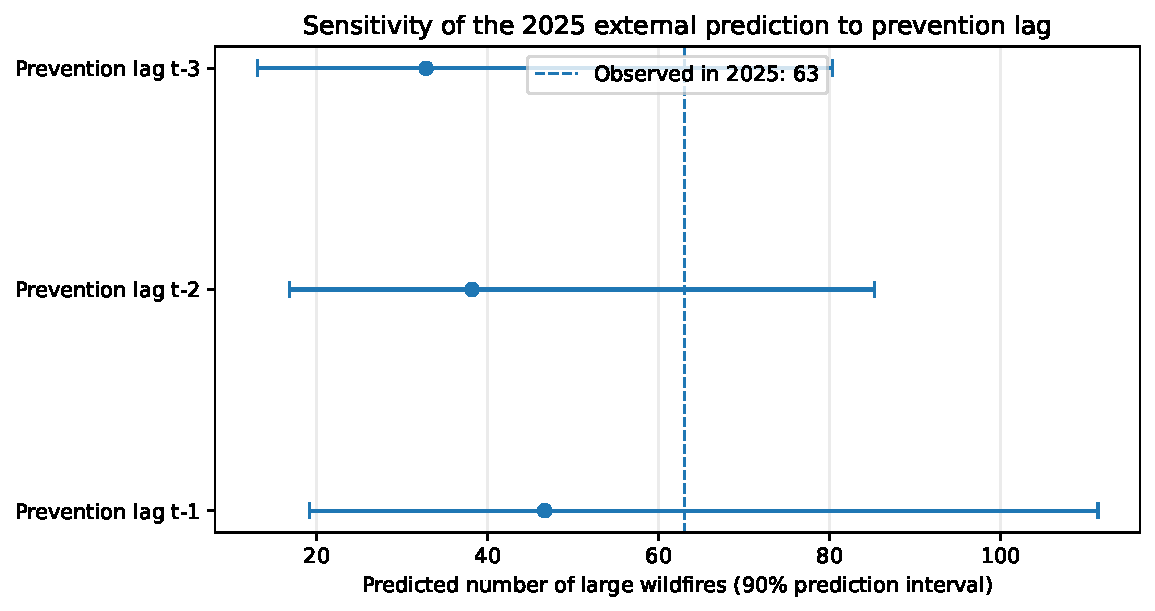
\includegraphics[width=0.82\textwidth]{../figures/figS2_2025_lag_sensitivity.pdf}
\caption{Sensitivity of the 2025 conditional prediction to the prevention lag.}
\end{figure}

\section{Prospective 2026 end-of-August snapshot}
The 2026 target was not incorporated into fitting or model selection. ARIMA$(1,0,0)$ was refitted using annual outcomes through 2025 and frozen before comparison with the provisional 2026 season.

\begin{table}[H]\centering\small
\begin{tabular}{lrrr}
\toprule
Quantity & Point/count & Lower & Upper \\
\midrule
Frozen ARIMA$(1,0,0)$ forecast & 17.44 & 4.62 & 59.54 \\
MITECO provisional, 2 Aug 2026 & 32 & --- & --- \\
MITECO/EFFIS estimate, 7 Aug 2026 & 39 & --- & --- \\
MITECO balance, 17 Aug 2026 & 42 & --- & --- \\
MITECO balance, 31 Aug 2026 & 44 & --- & --- \\
Historical completion benchmark from 44 & 49.9 & 45.9 & 68.5 \\
\bottomrule
\end{tabular}
\caption{Prospective 2026 snapshot. ARIMA limits are the 90\% prediction interval. The end-August completion benchmark applies the median and interquartile range of final-to-31-August count ratios from 2015--2024 and is descriptive, not a model forecast.}
\end{table}

The prospective sequence progressed from 32 large wildfires on 2 August to an EFFIS-supported estimate of 39 on 7 August, 42 in the mid-August MITECO balance and 44 in the national balance reported after the 31 August follow-up meeting. The corresponding end-August affected forest area was 264,656 ha. At 31 August 2025, the official MITECO report had recorded 60 large wildfires and an EFFIS-supported estimate of 346,443 ha. The 2015--2024 mean count at 31 August was 17.8. Applying the historical median final-to-31-August ratio (1.134) to the current 44 gives a descriptive completion value of 49.9 LWs (interquartile range 45.9--68.5); this is not a model forecast. All 2026 values remain provisional. The predictive lag-one ARIMAX requires 2025 prevention expenditure, which was unavailable in the harmonised series; the value was therefore left missing rather than imputed.

For sensitivity only, the lag-two log-linear equation can be evaluated conditionally because it uses the known 2024 prevention value (7.377 EUR ha$^{-1}$). The heat coefficient fitted through 2025 was 0.04843 per day ($p=0.00088$); the prevention coefficient was 0.10752 ($p=0.0612$), with retrospective $R^2_{\mathrm{fit,log}}=0.510$.

\begin{table}[H]\centering\small
\begin{tabular}{rrrr}
\toprule
2026 heatwave-day scenario & Predicted LWs & PI90 low & PI90 high \\
\midrule
20 & 25.61 & 9.06 & 69.38 \\
25 & 32.90 & 11.59 & 90.31 \\
30 & 42.19 & 14.59 & 118.69 \\
35 & 54.03 & 18.12 & 157.39 \\
40 & 69.10 & 22.25 & 210.38 \\
\bottomrule
\end{tabular}
\caption{Conditional 2026 heat-exposure scenarios from the lag-two inferential equation. These are not annual forecasts because the final 2026 heatwave-day total is not yet available.}
\end{table}

\section{Complete negative-binomial rolling validation}
{\scriptsize\setlength{\tabcolsep}{3pt}
\begin{longtable}{lrrrrrrrrr}
\toprule
Model & MAE & RMSE & NMAE & NRMSE & MASE & $R^2_{\mathrm{pred}}$ & MSE skill & CRPS & Coverage \\
\midrule
\endfirsthead
\toprule
Model & MAE & RMSE & NMAE & NRMSE & MASE & $R^2_{\mathrm{pred}}$ & MSE skill & CRPS & Coverage \\
\midrule
\endhead

Events + investment $(t-2)$ & 11.48 & 15.90 & 0.497 & 0.688 & 0.569 & 0.159 & 0.373 & 8.66 & 0.70 \\
Events + prevention $(t-2)$ & 14.40 & 17.57 & 0.624 & 0.761 & 0.714 & -0.028 & 0.234 & 10.14 & 0.60 \\
Endogenous & 16.70 & 20.07 & 0.723 & 0.869 & 0.827 & -0.341 & -0.000 & 10.43 & 0.90 \\
Investment $(t-2)$ & 14.97 & 20.18 & 0.648 & 0.874 & 0.742 & -0.356 & -0.011 & 10.87 & 0.80 \\
Prevention $(t-2)$ & 15.62 & 20.01 & 0.676 & 0.866 & 0.774 & -0.333 & 0.006 & 11.01 & 0.80 \\
Heat events & 28.05 & 38.43 & 1.214 & 1.664 & 1.389 & -3.916 & -2.665 & 15.11 & 0.80 \\
Heatwave days + prevention $(t-2)$ & 29.32 & 47.83 & 1.269 & 2.071 & 1.452 & -6.613 & -4.677 & 19.16 & 0.80 \\
\bottomrule
\end{longtable}
}

\section{Bayesian posterior summary}
\begin{table}[H]\centering\small
\begin{tabular}{lrrrrrr}
\toprule
Parameter & Mean & 2.5\% & 97.5\% & IRR & $P(<0)$ & $\widehat R$ \\
\midrule
Heatwave days (standardised) & 0.501 & 0.173 & 0.814 & 1.587 & 0.003 & 1.000 \\
Prevention $(t-2)$ (standardised) & 0.235 & -0.092 & 0.542 & 1.095 & 0.070 & 1.001 \\
Intercept & 2.984 & 2.661 & 3.314 & --- & 0.000 & 1.003 \\
AR(1) coefficient & -0.051 & -0.896 & 0.890 & --- & 0.547 & 1.007 \\
State SD & 0.283 & 0.016 & 0.684 & --- & 0.000 & 1.000 \\
Dispersion & 7.943 & 2.123 & 20.919 & --- & 0.000 & 1.001 \\
\bottomrule
\end{tabular}
\end{table}

On the natural scale, ten additional heatwave days had posterior IRR 1.587 (95\% credible interval 1.169--2.081). One additional real EUR ha$^{-1}$ of lag-two prevention had posterior IRR 1.095 (0.966--1.227).

\section{PCA loadings}
\begin{table}[H]\centering\small
\begin{tabular}{lrr}
\toprule
Variable & PC1 & PC2 \\
\midrule
Large-wildfire count & 0.574 & 0.783 \\
Heatwave days & 0.886 & 0.295 \\
Heatwave events & 0.911 & 0.240 \\
Prevention $(t-2)$ & -0.748 & 0.629 \\
Total investment $(t-2)$ & -0.606 & 0.758 \\
\bottomrule
\end{tabular}
\end{table}

PC1 and PC2 explained 54.0\% and 32.5\% of variance, respectively. Regional panel modelling and observational FWI integration are reserved for a separate follow-up study and are not presented as completed analyses in this supplement.

\end{document}
